\section{Question 2}

\subsection{Question}
\verbatiminput{q2/q2.txt}

\subsection{Answer}
The Edge Betweenness algorithm was run for target clusterings of three, four and five and the results are in Figures \ref{fig:cluster3}, \ref{fig:cluster4}, and \ref{fig:cluster5}.

\begin{figure}[h!]
\centering
\fbox{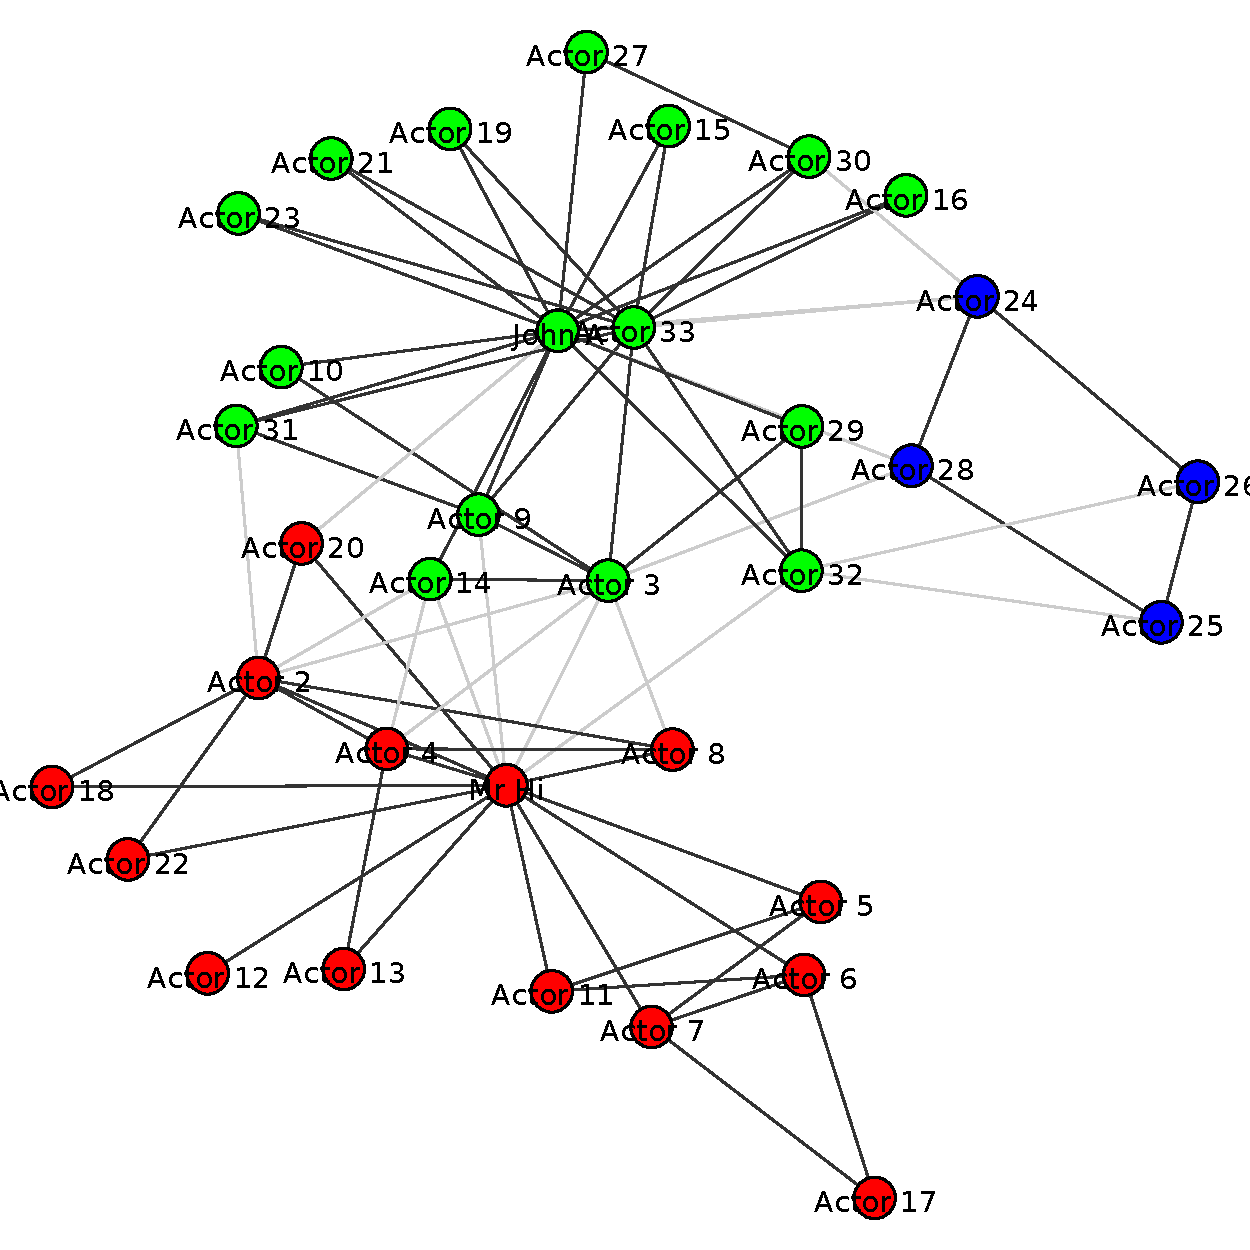
\includegraphics[scale=0.35]{q2/cluster3.pdf}}
\caption{3-Cluster Prediction}
\label{fig:cluster3}
\end{figure}

\begin{figure}[h!]
\centering
\fbox{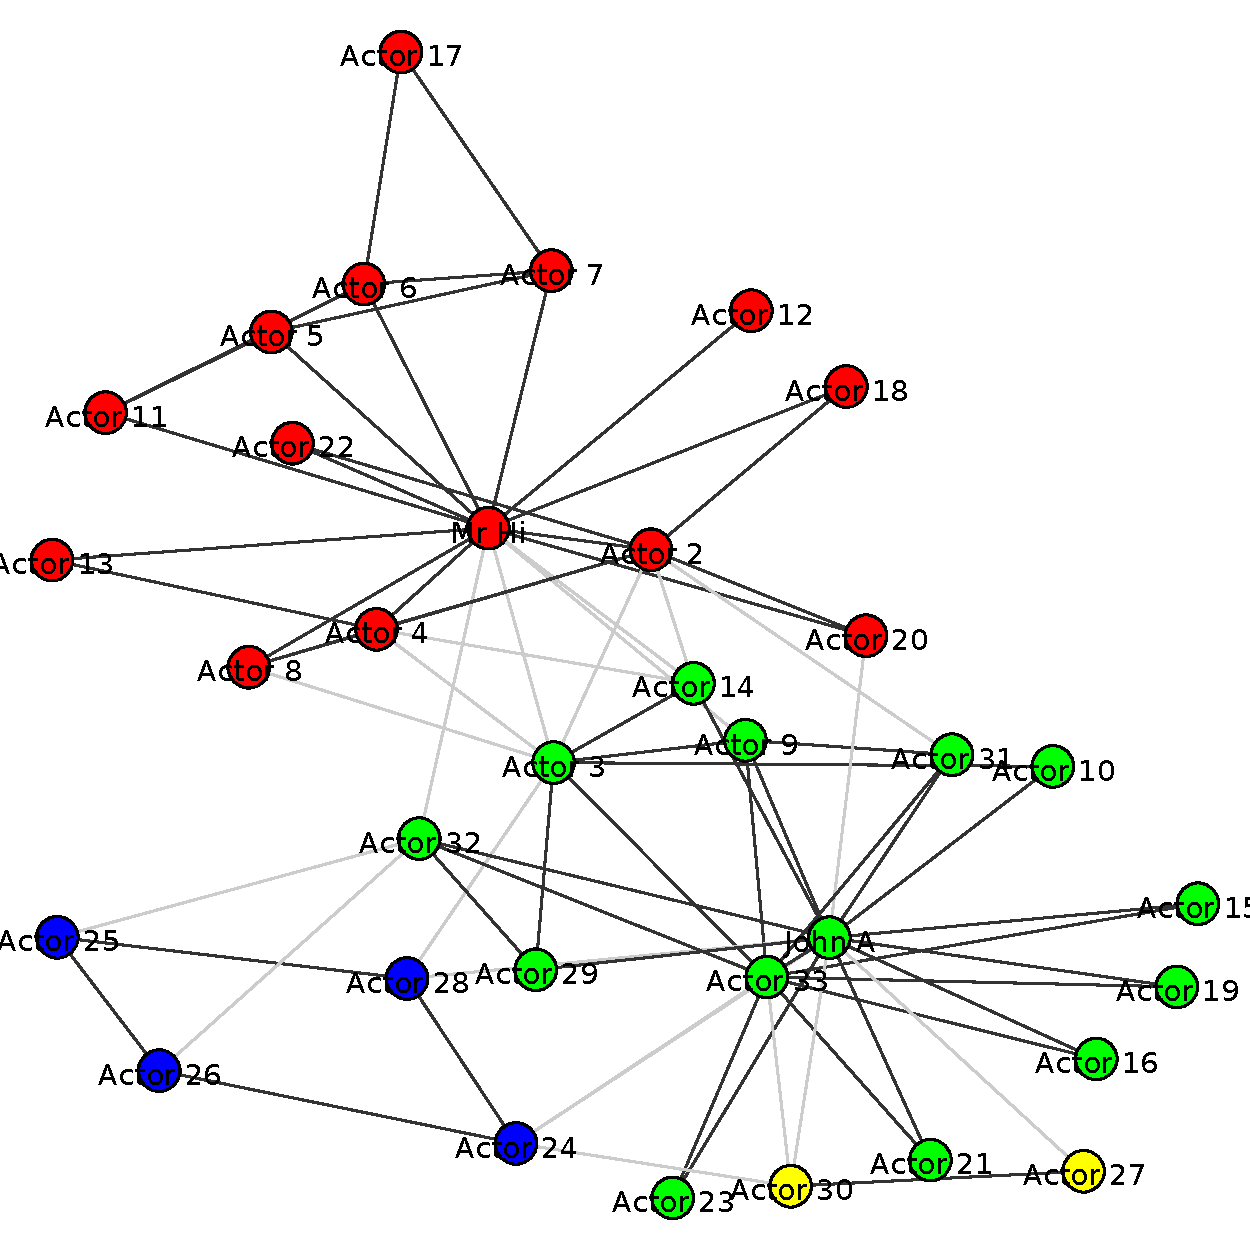
\includegraphics[scale=0.35]{q2/cluster4.pdf}}
\caption{4-Cluster Prediction}
\label{fig:cluster4}
\end{figure}

\begin{figure}[h!]
\centering
\fbox{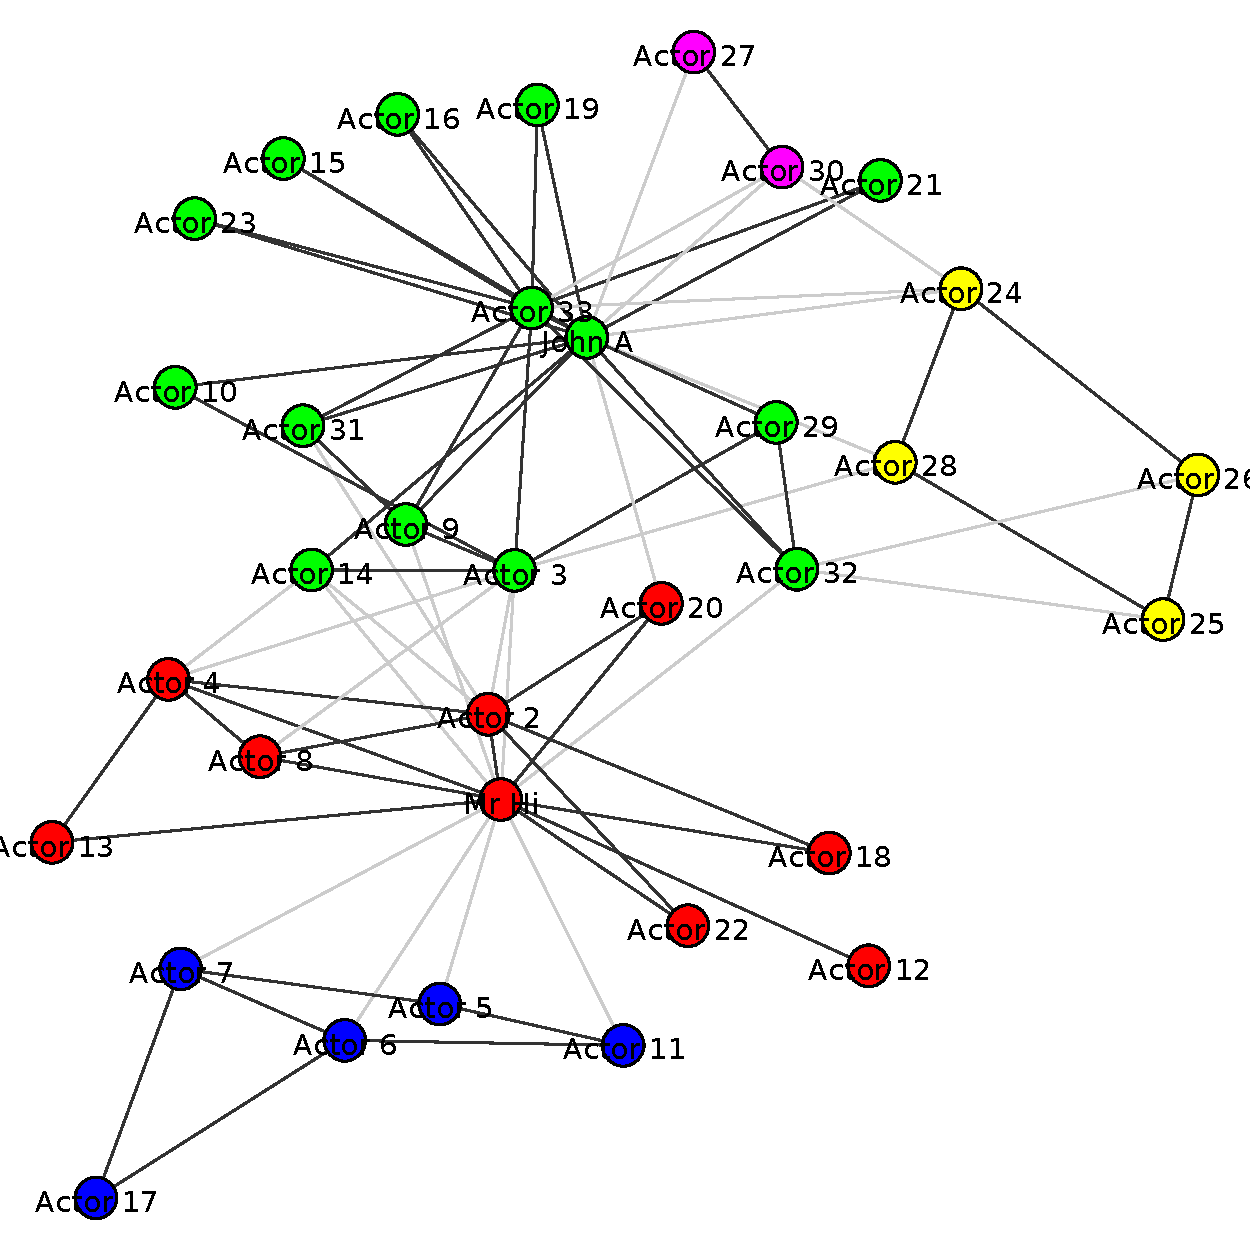
\includegraphics[scale=0.35]{q2/cluster5.pdf}}
\caption{5-Cluster Prediction}
\label{fig:cluster5}
\end{figure}